\documentclass{beamer}

\usepackage{amsmath,amssymb,amsthm}
\usepackage[all]{xy}
\usepackage{graphicx}



\numberwithin{equation}{subsection}

% Basic macros
\def\lim{\mathop{\mathrm{lim}}\nolimits}
\def\colim{\mathop{\mathrm{colim}}\nolimits}
\def\Spec{\mathop{\mathrm{Spec}}}
\def\Hom{\mathop{\mathrm{Hom}}\nolimits}
\def\Ext{\mathop{\mathrm{Ext}}\nolimits}
\def\Ker{\mathop{\mathrm{Ker}}}
\def\Im{\mathop{\mathrm{Im}}}
\def\Coker{\mathop{\mathrm{Coker}}}
 \def\Coim{\mathop{\mathrm{Coim}}}

% Slide numbering
\addtobeamertemplate{navigation symbols}{}{%
    \usebeamerfont{footline}%
    \usebeamercolor[fg]{footline}%
    \hspace{1em}%
    \insertframenumber/\inserttotalframenumber
}


\usepackage{tikz}
\usetikzlibrary{arrows.meta}

\title{Deformations of Stanley-Reisner schemes}
\author{Daniel González Casanova Azuela}
\institute{PUC-Rio}
\date{OPEGA\\ UFPE\\[1em] February 2026}

\begin{document}

\begin{frame}%Title page
\titlepage
\end{frame}


\section*{Plan of the talk}
\label{section-plan}

\begin{frame}%Plan of the talk
\frametitle{Plan of the talk}
\tableofcontents
\end{frame}


\section{Motivation}
\label{section-motivation}

\begin{frame}%Motivation
\frametitle{Motivation}

\noindent
{\color{blue}Kulikov, Persson, Roan (1970's):}
Let $\Sigma$ be the
dual complex associated to the normal crossing variety $X_0$,
the central fiber of a Kulikov degeneration of K3 surfaces.
Then the topological realization $|\Sigma|$ 
is either a point, an interval, or $S^2$ 
according to the type (I, II, III) of the degeneration.

\pause
\hspace{2em}

More generally,
$$
\xymatrix@C=4em{
\substack{\text{Hyperkähler} \\ \text{degeneration}}
\ar@{~>}[r]
&\substack{\text{SNC} \\ \text{special fiber}}
\ar@{~>}[r]
&\substack{\text{Dual complex $\Delta$,}\\
\text{rational homology $\mathbb{C}\mathbb{P}^n$}}
}
$$
\vspace{2.5em}

\end{frame}

\begin{frame}%Motivation
\frametitle{Motivation}

\noindent
{\color{blue}Kulikov, Persson, Roan (1970's):}
Let $\Sigma$ be the
dual complex associated to the normal crossing variety $X_0$,
the central fiber of a Kulikov degeneration of K3 surfaces.
Then the topological realization $|\Sigma|$ 
is either a point, an interval, or $S^2$ 
according to the type (I, II, III) of the degeneration.

\hspace{2em}

More generally,
$$
\xymatrix@C=4em{
\substack{\text{Hyperkähler} \\ \text{degeneration}}
\ar@{~>}[r]
&\substack{\text{SNC} \\ \text{special fiber}}
\ar@{~>}[r]
&\substack{\text{Dual complex $\Delta$,}\\
\text{rational homology $\mathbb{C}\mathbb{P}^n$}}
\ar@/^0.5pc/[dl]\\
& \substack{\text{Stanley-Reisner} \\ \text{scheme}}
\ar@/^.5pc/[lu]^{\text{smoothing} }
}
$$
\end{frame}


\begin{frame}%A triangulation of CP2
\frametitle{Strategy}

\iffalse
{\footnotesize
\begin{thebibliography}{1}
\bibitem{KuhnelBanchoff1983}
W. K{\"u}hnel and T. F. Banchoff,
\emph{The 9-vertex complex projective plane},
The Mathematical Intelligencer, 5(3) (1983), 11--22.
\end{thebibliography}
}\fi

\medskip\noindent
Smooth the SR scheme of the 9-vertex triangulation of $\mathbb{C}P^2$ 
discovered by Künhel-Banchoff.

\pause
\vspace{1em}
Start by smoothing the SR scheme of the {\bf link} of such triangulation,
an 8-vertex triangulation of $S^3$
called the Grünbaum sphere.

\medskip\noindent
\begin{figure}[H]
\centering
\centering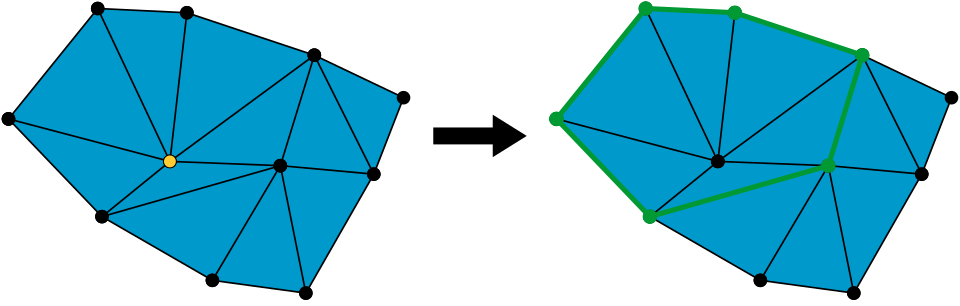
\includegraphics[width=0.7\textwidth]{link.png}
\caption{Link of a vertex in a simplicial complex}
\end{figure}
\end{frame}


\section{Objectives}

\begin{frame}%Objective
\frametitle{Objectives}
Short term:
\begin{itemize}
\item Show or disprove existence of a
Calabi-Yau threefold of degree 20 in $\mathbb{P}^7$
that degenerates to the Stanley-Reisner scheme of 
Grünbaum's triangulated 3-sphere with 8 vertices.
\end{itemize}
\pause

\vspace{2em}
Long term:
\begin{itemize}
\item Construct a degeneration
of generalized Kummer type fourfolds
with polarization degree 2
by smoothing the special fiber.
\end{itemize}
\end{frame}


\section{Definitions}
\begin{frame}%SR schemes
\frametitle{Stanley-Reisner schemes}
\begin{center}
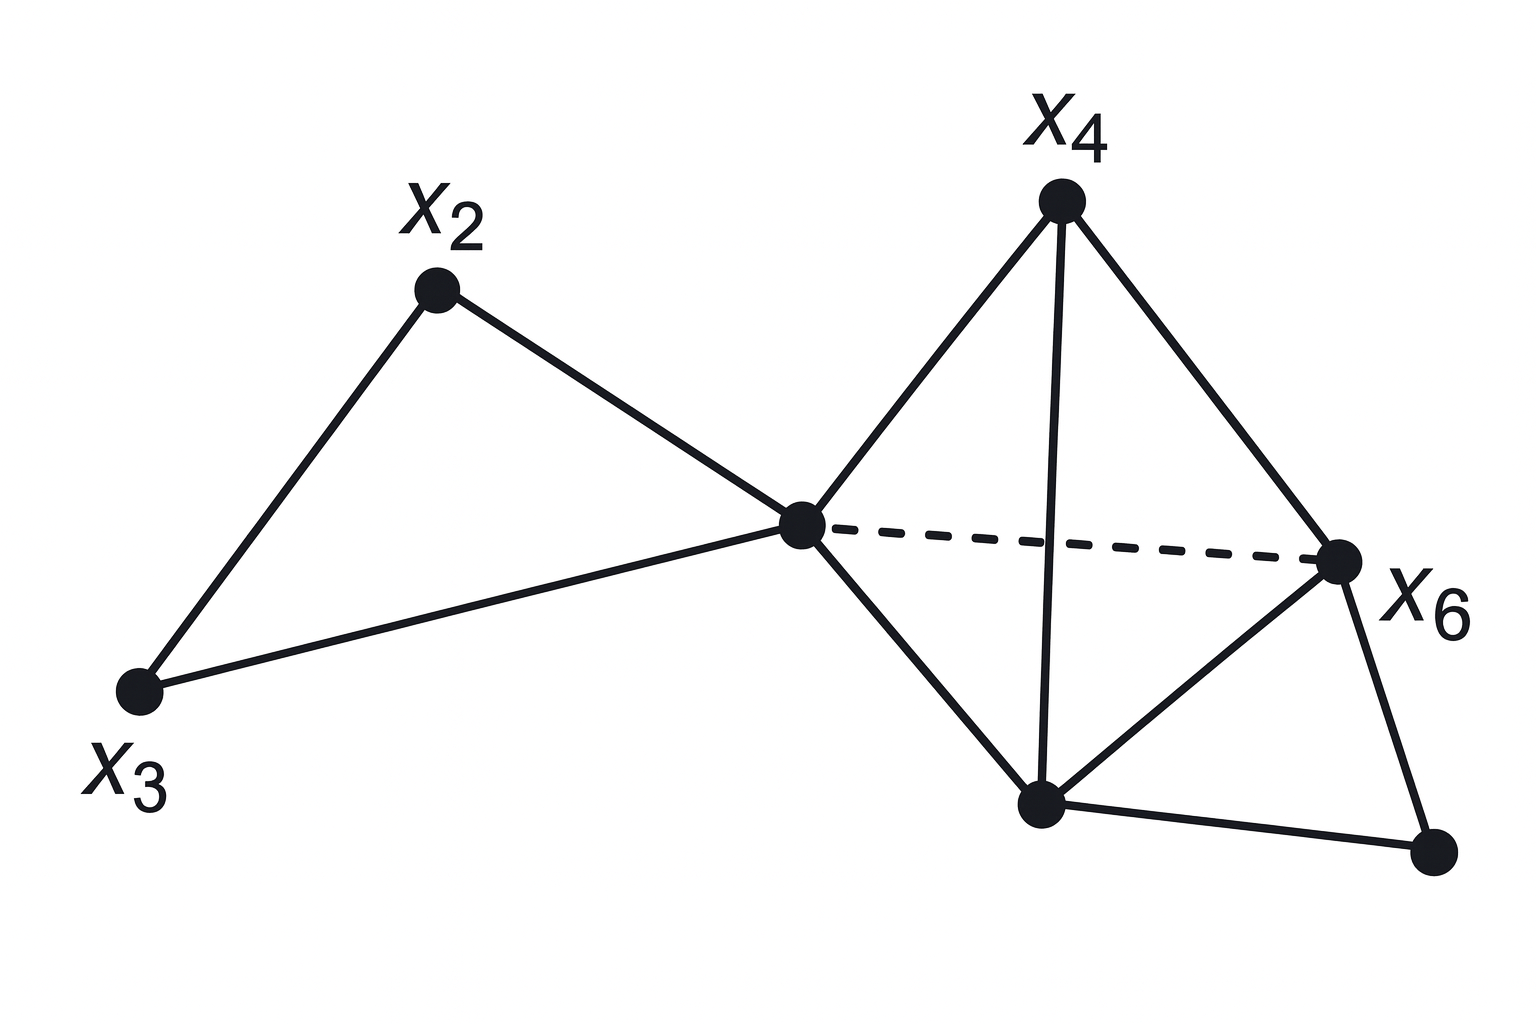
\includegraphics[width=.4\linewidth]{simplicial-complex.png}
\end{center}

The {\it Stanley-Reisner (SR) ideal}
of a simplicial complex $\mathcal{K}$ with $n$ vertices is
generated by the monomials in 
$R=\mathbb{C}[x_0,…,x_{n-1}]$
corresponding
to the ``non-faces'' of $\mathcal{K}$:
$$
I_{\mathcal{K}}=\left<x_p : p \in \Delta_n\setminus \mathcal{K}\right>.
$$
The {\it SR scheme} is $\text{Proj }R/I_{\mathcal{K}}$.
\end{frame}

\begin{frame}%Example: smoothing of a SR scheme
\frametitle{Example of a SR scheme}

Consider the
simplicial complex 
\begin{center}
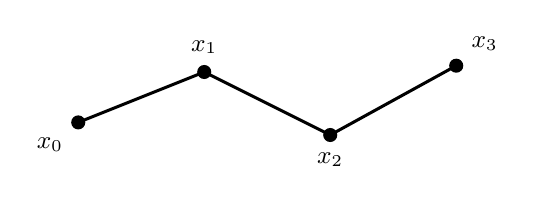
\begin{tikzpicture}[
  scale=.8,
  vertex/.style={circle, fill=black, inner sep=1.8pt},
  lab/.style={font=\small},
  edge/.style={line width=1.1pt}
]
  % vertices (fun angles)
  \coordinate (x0) at (0,0);
  \coordinate (x1) at (2,0.8);
  \coordinate (x2) at (4,-0.2);
  \coordinate (x3) at (6,0.9);

  % edges
  \draw[edge] (x0) -- (x1);
  \draw[edge] (x1) -- (x2);
  \draw[edge] (x2) -- (x3);

  % dots
  \node[vertex] at (x0) {};
  \node[vertex] at (x1) {};
  \node[vertex] at (x2) {};
  \node[vertex] at (x3) {};

  % labels (placed nicely)
  \node[lab, below left=2pt]  at (x0) {$x_0$};
  \node[lab, above=3pt]      at (x1) {$x_1$};
  \node[lab, below=3pt]      at (x2) {$x_2$};
  \node[lab, above right=2pt] at (x3) {$x_3$};
\end{tikzpicture}
\end{center}

Its SR ideal is generated by
$$
x_0x_2,\qquad x_0x_3,\qquad x_1x_3.
$$
\begin{tikzpicture}[
  panel/.style={draw, rounded corners=2pt, inner sep=6pt},
  comp/.style={line width=1.2pt},
  lab/.style={font=\small}
]

% ===== x1 = 1 (node) =====
\node[panel] at (0,0) {
\begin{tikzpicture}[scale=.5]
  % node (cross)
  \draw[comp] (-2,0) -- (2,0);
  \draw[comp] (0,-2) -- (0,2);
  \fill (0,0) circle (2pt);

  \node[lab] at (0,-2.7) {$x_1=1$};
\end{tikzpicture}
};

% ===== x0 = 1 (smooth line) =====
\node[panel] at (6,0) {
\begin{tikzpicture}[scale=.8]
  % smooth line
  \draw[comp] (-2.2,0) -- (2.2,0);

  \node[lab] at (0,-1.3) {$x_0=1$};
\end{tikzpicture}
};

\end{tikzpicture}

\end{frame}

\begin{frame}%Deformations
\frametitle{Deformations}
Let $X$ be scheme.
A {\it deformation} of $X$ is a Cartesian diagram 
$$
\xymatrix{
X\ar[r]\ar[d]&\mathcal{X}\ar[d]^{\pi}\\
\Spec \mathbb{C}\ar[r]&B
}
$$
where $\pi$ is a flat surjective morphism of algebraic $\mathbb{C}$-schemes and
$B$ is connected.

\medskip\noindent
A {\it smoothing} is a deformation where the general fibre $X_t$ 
of $\pi$ is smooth.
A {\it first order deformation} is a deformation 
where $B=\mathbb{C}[\varepsilon]/(\varepsilon^2)$,
which is an Artinian ring.
\end{frame}

\iffalse
\begin{frame}%Deformation of a hyperbola
\frametitle{Example: deformation of a hyperbola}
Consider the deformation
$$
\xymatrix{
\Spec\frac{\mathbb{C}[x,y]}{(xy-1)}\ar[r]\ar[d]
&\Spec\frac{\mathbb{C}[x,y,t]}{(xy-t)}\ar[d]\\
\Spec\frac{\mathbb{C}[t]}{(t-1)}\ar[r]
&\Spec \mathbb{C}[t]
}
$$
where $\pi:\mathcal{X} \to B$ be the morphism
determined by the natural homomorphism
$\mathbb{C}[t] \to \mathbb{C}[x,y,t]/(ty-x^2)$.

\medskip\noindent
The generic fibre is a (smooth) hyperbola 
while the fibre at $t=0$ is singular and reducible.
\end{frame}
\fi

\begin{frame}
\begin{tikzpicture}[
  panel/.style={draw, rounded corners=2pt, inner sep=6pt},
  comp/.style={line width=1.2pt},
  lab/.style={font=\small}
]

% ===== left: node =====
\node[panel] at (0,0) {
\begin{tikzpicture}[scale=.85]
  % axes (optional but helps)
  \draw[->] (-2.3,0) -- (2.3,0);
  \draw[->] (0,-2.3) -- (0,2.3);

  % node: x0 x2 = 0
  \draw[comp] (-2,0) -- (2,0);
  \draw[comp] (0,-2) -- (0,2);
  \fill (0,0) circle (2pt);

  \node[lab] at (0,-2.75) {$x_1=1$ (node)};
\end{tikzpicture}
};

% arrow
\draw[->, line width=0.9pt] (2.7,0) -- (3.9,0);

% ===== right: hyperbola =====
\node[panel] at (6.5,0) {
\begin{tikzpicture}[scale=.85]
  % axes
  \draw[->] (-2.3,0) -- (2.3,0);
  \draw[->] (0,-2.3) -- (0,2.3);

  % hyperbola: x0 x2 + 1 = 0  i.e. x2 = -1/x0
  % plot away from 0 on both sides
  \draw[comp, domain=-2.2:-0.35, samples=200]
    plot (\x, {-1/(\x)});
  \draw[comp, domain=0.35:2.2, samples=200]
    plot (\x, {-1/(\x)});

  \node[lab] at (0,-2.75) {$x_1=1$ (smoothed)};
\end{tikzpicture}
};
\end{tikzpicture}

\noindent
Consider instead
\begin{align*}
x_0x_2\xymatrix{\ar@{~>}[r]&}&x_0x_2+{\color{red}t}x_1^2\\
x_0x_3\xymatrix{\ar@{~>}[r]&}&x_0x_3\\
x_1x_3\xymatrix{\ar@{~>}[r]&}&x_1x_3+{\color{red}s}x_2^2
\end{align*}

\end{frame}

\section{Smoothing method 1: Artin's criterion for flatness}
\label{section-artin}

\begin{frame}%Method 1
\frametitle{Smoothing method 1}

\begin{theorem}[Artin's criterion for flatness]
\label{theorem-artin-criterion}
Let $R=\mathbb{C}[x_1,…,x_n]$.
Let $A$ be a local Artinian algebra of finite type over $\mathbb{C}$.
Let $I \subset R$ and $I_A \subset R_A:=R\otimes A$.
Suppose that there is an exact sequence

\begin{equation}
\label{equation-artin-criterion1}
\xymatrix{
R^\ell\ar[r]
&R^m\ar[r]
&R\ar[r]
&R/I\ar[r]
&0
}
\end{equation}

\noindent
and a complex
\begin{equation}
\label{equation-artin-criterion2}
\xymatrix{
R^\ell_A\ar[r]
&R^m_A\ar[r]
&R_A\ar[r]
&R_A/I_A\ar[r]
&0
}
\end{equation}

\noindent
such that the part
$$
\xymatrix{
R^m_A\ar[r]
&R_A\ar[r]
&R_A/I_A\ar[r]
&0
}
$$
is exact. 
Then, if
(\ref{equation-artin-criterion2})$\otimes_A\mathbb{C}
=$(\ref{equation-artin-criterion1}),
the module $R_A/I_A$ is $A$-flat.
\end{theorem}
\end{frame}

\begin{frame}%In our example
\frametitle{Smoothing method 1 (toy example)}

{\color{blue}Step 1:} write deformation polynomials
\begin{align*}
I\qquad &\qquad \qquad I \otimes A
= I \otimes \mathbb{C}[a_1,…, a_6,b_1,…,b_6,c_1,…,c_6]/\sim
\\
\hspace{-0.5em}f_1:=x_0x_2&\xymatrix{\ar@{~>}[r]&}
x_0x_2+a_0x_0^2+a_1x_0x_1+a_2x_1^2+a_3x_1x_2+a_4x_2^2+a_5x_2x_3+a_6x_3^2\\
f_2:=x_0x_3&\xymatrix{\ar@{~>}[r]&}
x_0x_3+b_0x_0^2+b_1x_0x_1+b_2x_1^2+b_3x_1x_2+b_4x_2^2+b_5x_2x_3+b_6x_3^2\\
f_3:=x_1x_3&\xymatrix{\ar@{~>}[r]&}
x_1x_3+c_0x_0^2+c_1x_0x_1+c_2x_1^2+c_3x_1x_2+c_4x_2^2+c_5x_2x_3+c_6x_3^2
\end{align*}

\pause\noindent
{\color{blue}Step 2:} find the syzygies of $I$:
$$
-x_3 f_1+x_2f_2=0,\qquad  \text{and}\qquad 
-x_1f_2+x_0f_3=0.
$$


\pause\medskip\noindent
{\color{blue}Step 3:} impose syzygy conditions on $I\otimes A$
and simplify
$$
a_4=b_5,\quad  a_5=b_6,
\quad b_0=c_1, \quad  b_1=c_2,
\quad a_6=b_2=b_3=b_4=c_0=0.
$$
(exactly 12 free variables!)
\end{frame}


\begin{frame}%Smoothing method 1 (toy example)
\frametitle{Smoothing method 1 (toy example)}
{\color{blue}Step 4:} find a smooth fiber using Jacobian criterion

In fact, our earlier guess
$$
x_0x_2\xymatrix{\ar@{~>}[r]&}x_0x_2+{\color{red}t}x_1^2\qquad 
x_0x_3\xymatrix{\ar@{~>}[r]&}x_0x_3\qquad 
x_1x_3\xymatrix{\ar@{~>}[r]&}x_1x_3+{\color{red}s}x_2^2
$$
is a valid choice.

\vspace{2em}{\color{blue}Step 5:} check for obstructions.

The deformation space of curves is unobstructed.
\end{frame}


\begin{frame}%Smoothing method 1 (actual problem)
\frametitle{Smoothing method 1 (actual problem)}

\begin{itemize}
\item There are 
16 degree-3 
monomials in $\mathbb{C}[x_0,…,x_7]$ generating the ideal of
the Stanley-Reisner scheme of Grünbaum's sphere.

\item There are 16*104 deformation variables 
$a_1,…,a_{104}, b_1,…,b_{104},…,p_1,…,p_{104}$.

\item Found 1555 syzygy constraints which simplify the polynomials.

\item Did not find a smooth fibre using Jacobian criterion so far.

\item Obstructions?
\end{itemize}

\end{frame}

\section{Smoothing method 2: Gröbner degenerations}
\label{section-grobner}

\begin{frame}%Another method: starting from the smooth fiber
\frametitle{Smoothing method 2 (toy example)}
\begin{center}
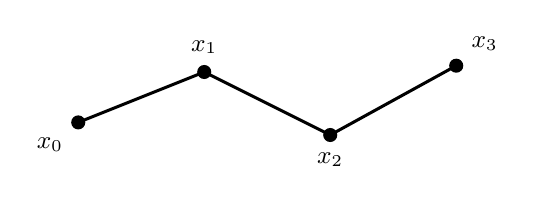
\begin{tikzpicture}[
  scale=.8,
  vertex/.style={circle, fill=black, inner sep=1.8pt},
  lab/.style={font=\small},
  edge/.style={line width=1.1pt}
]
  % vertices (fun angles)
  \coordinate (x0) at (0,0);
  \coordinate (x1) at (2,0.8);
  \coordinate (x2) at (4,-0.2);
  \coordinate (x3) at (6,0.9);

  % edges
  \draw[edge] (x0) -- (x1);
  \draw[edge] (x1) -- (x2);
  \draw[edge] (x2) -- (x3);

  % dots
  \node[vertex] at (x0) {};
  \node[vertex] at (x1) {};
  \node[vertex] at (x2) {};
  \node[vertex] at (x3) {};

  % labels (placed nicely)
  \node[lab, below left=2pt]  at (x0) {$x_0$};
  \node[lab, above=3pt]      at (x1) {$x_1$};
  \node[lab, below=3pt]      at (x2) {$x_2$};
  \node[lab, above right=2pt] at (x3) {$x_3$};
\end{tikzpicture}
$I= \left<x_0x_2,x_0x_3,x_1x_3\right>$
\end{center}

The twisted cubic is a smoothing of this variety.
Recall that the {\it twisted cubic} is the image 
of the Veronese map of degree 3,
\begin{align*}
\nu: \mathbb{P}^1 &\longrightarrow \mathbb{P}^3 \\
[u:v] &\longmapsto [u^3:u^2v:uv^2:v^3]=[x_0:x_1:x_2:x_3],
\end{align*}
and its ideal is generated by
$$
x_1^2-x_0x_2,\quad x_1x_2-x_0x_3,\quad x_2^2-x_1x_3.
$$
\end{frame}


\begin{frame}%Another method: starting from the smooth fiber
\frametitle{Smoothing method 2 (toy example)}
This time introduce only {\bf one} new variable $t$ 
and four constants:
$$
x_0\rightsquigarrow t^ax_0,\qquad 
x_1\rightsquigarrow t^bx_1,\qquad 
x_2\rightsquigarrow t^cx_2,\qquad 
x_3\rightsquigarrow t^dx_3.
$$
The equations of the twisted cubic become
$$
\xymatrix{
x_1^2-x_0x_2,\ar@{~>}[d]
&x_1x_2-x_0x_3,\ar@{~>}[d]
&x_2^2-x_1x_3\ar@{~>}[d]\\
t^{2b}x_1^2-t^{a+c}x_0x_2,
&t^{b+c}x_1x_2-t^{a+d}x_0x_3,
&t^{2c}x_2^2-t^{b+d}x_1x_3.
}
$$
\pause
We try to kill the spare terms to arrive at our ideal as $t \to 0$
\begin{align*}
2b>a+c,\qquad b+c>a+d,\qquad 2c>b+d.
\end{align*}
A solution is $a=1,b=2,c=2,d=0$.
\end{frame}


\begin{frame}%Gröbner degenerations
\frametitle{Smoothing method 2: Gröbner degenerations}

Let $R=\mathbb{C}[x_0,…,x_n]$.
and fix a vector $\omega=(\omega_1,\ldots,\omega_n)\in\mathbb{R}^n$.
Let $f=\sum c_a x^a \in R$
and $b:=\text{max}\{\omega\cdot a:c_a \neq 0\}$.
The {\it homogenization of $f$} is
$$
\tilde{f}:=\sum c_a x^a t^{b-\omega\cdot a} \in R[t]
$$
and the {\it homogenization ideal $\tilde{I}\subset R[t]$} 
is the ideal generated by the $\tilde{f}$ for $f$ in an ideal $I\subset R$.

\vspace{1em}
The {\it initial form $\text{in}_\omega(f)$ of $f$} is
the sum of all terms
$c_ix^{a_i}$ such that the inner product $\omega\cdot a_i$
is maximal. 
The {\it initial ideal} of $I$ is the ideal
generated by all initial forms.
\end{frame}

\begin{frame}%Gröbner degenerations
\frametitle{Smoothing method 2: Gröbner degenerations}

\begin{theorem}[Eisenbud, Commutative Algebra with a view…]
\label{theorem-grobner-flat-morphism}
For any ideal $I \subset k[x_1,\ldots,x_r]:=S$, the
$k[t]$-algebra $S[t]/\tilde{I}$ is free ---and thus flat---
as a $k[t]$ module. […]
\iffalse$$
S[t]/\tilde{I}\otimes_{k[t]}k[t,t^{-1}]
\cong S[t]/I[t,t^{-1}],
$$
while
$$
S[t]/\tilde{I}\otimes_{k[t]}k[t]/(t)
\cong S[t]/\text{in}_{\omega}(I).
$$\fi

\vspace{2em}
Thus $S[t]/\tilde{I}$ is a flat family over $k[t]$ of quotients
of $S$ whose fiber over $0$ is $S/\text{in}_\omega(I)$ and
whose fiber over any $(t-u)$ for $0 \neq u \in k$ is $S/I$.
\end{theorem}


\end{frame}

\begin{frame}%Gröbner degenerations
\frametitle{Smoothing method 2 (toy example)}
\vspace{-2em}
$$
\begin{array}{cccc}
\text{SR}(\bullet-\bullet-\bullet-\bullet) & x_0x_2, & x_0x_3, & x_1x_3 \\
\text{twisted cubic} 
& x_1^2-x_0x_2, & x_1x_2-x_0x_3, & x_2^2-x_1x_3.
\end{array}
$$
Consider the weight vector $\omega=(5,-5,-5,5)$.
The inner products of $\omega$ with the vectors $\mathbf{a}_i$
in the generators of the ideal for the twisted cubic are
\begin{align*}
\omega\cdot(0,2,0,0)&=-10,\qquad \omega\cdot(1,0,1,0)=0\\
\omega\cdot(0,1,1,0)&=-10,\qquad \omega\cdot(1,0,0,1)=10\\
\omega\cdot(0,0,2,0)&=-5,\qquad \omega\cdot(0,1,0,1)=0
\end{align*}

\noindent
The initial ideal is the ideal of the SR scheme.
\end{frame}


\iffalse
\begin{frame}%Grünbaum sphere
\frametitle{Grünbaum sphere}

{\footnotesize
\begin{thebibliography}{1}
\bibitem{grun}
B. Grünbaum and V.~P. Sreedharan,
\emph{An enumeration of simplicial 4-polytopes with 8 vertices},
J. Combin. Theory, 2 (1967), 437–465.
\end{thebibliography}
}

\medskip\noindent
Grünbaum-Shreedharan discovered a simplicial complex $\mathcal{M}$ 
which is not the boundary of a 4-polytope
despite being a triangulation of the 3-sphere.

\pause\medskip\noindent
A smoothing of $\text{SR}(\mathcal{M})$ would
be a CY 3-fold of degree 20 in $\mathbb{P}^7$:
\begin{lemma}
\label{lemma-degree}
The number of maximal facets of a triangulation equals the
degree of the associated variety.
\end{lemma}

\begin{theorem}
\label{theorem-smoothing-triangulation}
If it exists, a smoothing of the SR scheme of a 
triangulation of the 3-sphere yields a Calabi-Yau threefold.
\end{theorem}

\noindent
\end{frame}\fi

\begin{frame}%A smooth candidate
\frametitle{Smoothing method 2 (actual problem)}

There exists a CY threefold in $\mathbb{P}^7$ of degree
20 that was first studied 
by Gulliksen-Neg\aa ard.
Its ideal is generated by the
$3\times 3$ minors of $4\times 4$ matrix with linear forms.

\medskip\noindent
For example,
$$
\begin{bmatrix}
x_1 & x_2 & x_3 & x_4 \\
x_5 & x_6 & x_7 & x_8 \\
x_2 & x_3 & x_4 & x_5 \\
x_6 & x_7 & x_8 & x_1
\end{bmatrix}
$$
\end{frame}

\begin{frame}%
\frametitle{Smoothing method 2 (actual problem)}
\vspace{-1em}{\tiny
\begin{align*}
\text{SR}(\mathcal{M})\qquad \qquad & 
\qquad \qquad \qquad \qquad \qquad \quad \text{GN}\\ 
x_6x_7x_8,\qquad \qquad 
&x_3^2 x_5 - x_2 x_4 x_5 - x_2 x_3 x_6 + x_1 x_4 x_6 + x_2^2 x_7 - x_1 x_3 x_7, \\
x_4x_6x_8,\qquad \qquad &-x_3 x_6^2 + x_3 x_5 x_7 + x_2 x_6 x_7 - x_1 x_7^2 - x_2 x_5 x_8 + x_1 x_6 x_8, \\
x_3x_7x_8,\qquad \qquad &-x_3^2 x_6 + x_2 x_4 x_6 + x_2 x_3 x_7 - x_1 x_4 x_7 - x_2^2 x_8 + x_1 x_3 x_8, \\
x_3x_5x_7,\qquad \qquad &x_4 x_6^2 - x_4 x_5 x_7 - x_3 x_6 x_7 + x_2 x_7^2 + x_3 x_5 x_8 - x_2 x_6 x_8, \\
x_3x_4x_8,\qquad \qquad &x_3 x_4 x_5 - x_2 x_5^2 - x_2 x_4 x_6 + x_1 x_5 x_6 + x_2^2 x_8 - x_1 x_3 x_8, \\
x_2x_7x_8,\qquad \qquad 
&-x_1 x_2 x_5 + x_1^2 x_6 - x_4 x_6^2 + x_4 x_5 x_7 + x_2 x_6 x_8 - x_1 x_7 x_8, \\
x_2x_5x_7,\qquad \qquad 
&-x_1 x_2^2 + x_1^2 x_3 - x_3 x_4 x_6 + x_2 x_5 x_6 + x_2 x_4 x_7 - x_1 x_5 x_7, \\
x_2x_5x_6,\qquad \qquad 
&x_1 x_3 x_5 - x_1 x_2 x_6 + x_5 x_6^2 - x_5^2 x_7 - x_3 x_6 x_8 + x_2 x_7 x_8, \\
x_2x_4x_7,\qquad \qquad 
&x_4^2 x_5 - x_3 x_5^2 - x_2 x_4 x_7 + x_1 x_5 x_7 + x_2 x_3 x_8 - x_1 x_4 x_8, \\
x_2x_4x_6,\qquad \qquad 
&-x_1 x_3 x_5 + x_1^2 x_7 - x_4 x_6 x_7 + x_4 x_5 x_8 + x_3 x_6 x_8 - x_1 x_8^2, \\
x_1x_4x_6,\qquad \qquad 
&-x_1 x_2 x_3 + x_1^2 x_4 - x_4^2 x_6 + x_3 x_5 x_6 + x_2 x_4 x_8 - x_1 x_5 x_8, \\
x_1x_4x_5,\qquad \qquad 
&x_1 x_4 x_5 - x_1 x_2 x_7 + x_5 x_6 x_7 - x_5^2 x_8 - x_4 x_6 x_8 + x_2 x_8^2, \\
x_1x_3x_8,\qquad \qquad 
&x_4^2 x_6 - x_3 x_5 x_6 - x_3 x_4 x_7 + x_2 x_5 x_7 + x_3^2 x_8 - x_2 x_4 x_8, \\
x_1x_3x_6,\qquad \qquad 
&-x_1 x_3 x_6 + x_1 x_2 x_7 - x_4 x_7^2 + x_4 x_6 x_8 + x_3 x_7 x_8 - x_2 x_8^2, \\
x_1x_3x_5,\qquad \qquad 
&-x_1 x_3^2 + x_1 x_2 x_4 - x_4^2 x_7 + x_3 x_5 x_7 + x_3 x_4 x_8 - x_2 x_5 x_8, \\
x_1x_2x_5,\qquad \qquad 
&x_1 x_4 x_6 - x_1 x_3 x_7 + x_5 x_7^2 - x_5 x_6 x_8 - x_4 x_7 x_8 + x_3 x_8^2
\end{align*}}
\end{frame}

\section*{References}
\label{section-ref}

\begin{frame}%References
\frametitle{References}

{\scriptsize
\begin{thebibliography}{1}


\bibitem{KollarLazaSaccaVoisin2018}
J. Koll\'ar, R. Laza, G. Sacc\`a, and C. Voisin,
\emph{Remarks on degenerations of hyper-K\"ahler manifolds},
arXiv:1704.02731 (2018).

\bibitem{KuhnelBanchoff1983}
W. K{\"u}hnel and T. F. Banchoff,
\emph{The 9-vertex complex projective plane},
The Mathematical Intelligencer, 5(3) (1983), 11--22.

\bibitem{grun}
B. Grünbaum and V.~P. Sreedharan,
\emph{An enumeration of simplicial 4-polytopes with 8 vertices},
J. Combin. Theory, 2 (1967), 437–465.

\bibitem{callatalk}
C. Tschanz,
\emph{Talk at Kummers in Kraków (2024)},
\url{https://www.callatschanz.com/talks-and-travels}.

\bibitem{Fausk}
I. Fausk,
\emph{Pfaffian Calabi-Yau threefolds, Stanley-Reisner schemes and mirror symmetry},
PhD thesis, 2012.

\bibitem{AlecciMichele2025}
G. Alecci and M. Graffeo,
\emph{Computations in Algebraic Geometry},
Course notes, IMECC/UNICAMP, Campinas/SP (March 2025).\\
\url{https://graffeomichele.github.io/NotesCiAG.pdf}

\bibitem{Eisenbud}
D. Eisenbud,
\emph{Commutative Algebra: With a View Toward Algebraic Geometry},
Springer, 1995.

\end{thebibliography}
}

\end{frame}

\begin{frame}%Thank you
\centering
\LARGE Obrigado!
\end{frame}

\bibliography{my}
\bibliographystyle{amsalpha}

\end{document}
